\documentclass[12pt,a4paper]{article}

\usepackage{epcc}
%\usepackage{graphics}
\usepackage{graphicx}
\usepackage{pgfgantt}
\usepackage{array}

% This example file shows how a thesis can be laid out using Latex. It
% does not use any special local features so should be portable to other
% places.
%
% To produce myfile.pdf from myfile.tex type:
% 
% pdflatex myfile
%
% Note that pdflatex expects all included figures to be in PDF too. See
% the includegraphics command below.


% This document contains many cross-references and forward references,
% eg in constructing a table of contents, so Latex may need to be run
% twice to get all the references correct. If you need to run Latex twice
% you may get the warning:
% 
% LaTeX Warning: Label(s) may have changed. Rerun to get cross-references right


\begin{document}

\title{Software Development\\UI and Evaluation Plan}
\author{B098688 - s1671778}
\date{\today}

\makeEPCCtitle

\thispagestyle{empty}

\newpage

\pagenumbering{roman}

\tableofcontents


\newpage
\pagenumbering{arabic}

\section{Introduction}

This report will go through choices made to improve a provided semi-functional web interface (implemented in HTML and JavaScript) of a ``squad roster builder for a tabletop miniatures skirmish game, a type of war game''~\cite{soft_dev}. The given interface has multiple problems, some of which were addressed in the previous report. Nonetheless, they will be explained again in a succinct manner. The main problem that the given program has is that it is extremely alienating for its user. This is why a mock-up of an improved design is provided in this report. Said mock-up attempts to address the problems while keeping true to customer demands and requirements. 

The first part of this report will outline the problems encountered with the given interface together with an explanation on why they constitute problems to its functionality and user-friendliness. The end of the section will include a short text on how these problems should be attacked and ultimately solved. This does not mean that all the problems were encountered, nor that they were resolved in the best way - the report will come back to this in the last section.

The attempts at a solution for said problems are outlined in the second section. These are presented both in a visual and textual manner. The images used are mock-ups of the proposed solutions using the web-based tool Mybalsamiq. These show various pages for the improved web application and some explanatory comments. The solutions attempt to mimic what other web pages have established as norm (for example login and logout options on the top right corner of the web page).

The third, and final, section describes a proposed way for evaluating the proposed changes to the given interface. These cover a range of potential users, as well as the client and people who have interests in other, similar, war games. The complete evaluation plan will attempt to discover even more problems with the revised interface. The end goal of these evaluation procedures is to make the web application more user-friendly and users want to come back to it.

The most important improvement that can be made on the current web application as far as user interface (UI) and design choices is the addition of a multiple user functionality. This is required according to the client's specifications. A registration process will be included with the approach used to solve this problem and it is proposed to include a chatting/messaging functionality to allow users to interact among themselves. This could be an interesting tool as it would let the users arrange meetings to play the game.

After setting up the multiple user interface, it is possible to fulfill the game's requirements regarding public/private warbands (squads). That is, allow all players to view public warbands but only the owner can edit it, and only the owner to view their private warbands. A problem that is underlying in the solutions that have been provided is the addition of some colour to the webpage. This will help in making the application more user friendly and generally appealing.

\section{Design an UI Problems}
\label{sec:concept}

This section lays out the problems that have been identified in the given web application (that has been written in HTML and JavaScript). Said problems are divided in various sections and are ordered on a basis of importance (the first being the most important). Briefly, the problems encountered fall into one or more of the following categories: multiple user support (that is a customer requirement), navigation (such that the application is easy-to-use and user-friendly), error handling (for attempts to create invalid warbands or similar errors), confirmation messages (preventing when actions will be irreversible), game information, rules, and other problems. 

\subsection{Multiple User Support}

The most extensive, and far reaching, problem is that the provided web application does not support multiple users. This is one of the client demands: the application ``should allow for a player to delete their own warbands but not those of another player. Additionally players should not be allowed to view other players' warband unless the warband has been marked public.'' This means that the improved web application must have:

\begin{enumerate}
 \item Multiple user support.
 \item A way for users to dictate whether they want to have public or private warbands.
 \item A way for users to view, but not edit, other user's public warbands. 
\end{enumerate}

This problem should be attacked in the early stages of translating design to a real, functional, web application. This is due to the fact that the multiple user issue seeps into other problems.

\subsection{Navigation Problems}

Another of the main problems that were found with the provided web application was the difficulty with navigating through pages. For example:

\begin{enumerate}
 \item Impossible to navigate to the home page after successfully creating a new warband (squad). The only way to reach the home page after doing so was to use the address bar and type the home page's location. This would be an extremely annoying problem that a user would definitely encounter.
 \item A second navigation problem was that if the user attempted to create an invalid warband the application would take them to an error page that, again, was impossible to leave without using the address bar.
\end{enumerate}

\subsection{Error Handling}

The problem regarding error handling was already mentioned in the previous report, and it is worth while mentioning it once more as it directly relates to proper design choices. While using the given interface the appearance of error messages was extremely bothersome. 

When attempting to make an illegal warband, or when doing so unintentionally, a generic error message (fig.~1) appeared that provided no information regarding the reason behind it, or means to return to the previous page. 

\begin{figure}[h]
 \centering
 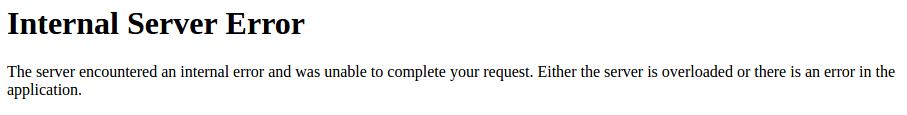
\includegraphics[width=1\textwidth]{img/warband_error}
 \label{fig:1}
 \caption{Generic error message.}
\end{figure}

\begin{enumerate}
 \item The error message provides no information as to why it appeared. This would be frustrating for someone attempting to create an illegal warband, but not knowing what was the problem with it. 
 \item Once the error message appears there is no ``Return'', ``Back'', or ``Home'' button to leave the error message page. 
 \item The only way to return to the web application is to use the address bar. This is profoundly alienating for new users.
 \item There is no error, or even message, to warn about creating a warband with a name that is already in use. 
\end{enumerate}

The main method for trying to fix this problem is reducing the times where error messages appear. Instead using messages explaining why the action that a user wants to do is not supported and how to fix it. The next section will delve further into this.

\subsection{Confirmation Messages}

Deleting a warband is an irreversible action. So is removing members from a warband while it is being edited. When a user attempt to do one of these actions there is no message warning them on the consequences. 

\begin{enumerate}
 \item The game rules state that when editing a warband if one of its members is removed the credits used to hire them are not returned to the warband's bank. This can be unknown to the user, but suffer from removing a character by accident or by purposefully doing so and expecting an increase in credits.
 \item The user can delete one of their warbands with only one click. This can happen by accident and is an irreversible action. This ought to be more user-friendly.
\end{enumerate}

These actions could be fixed by introducing confirmation messages and/or ``Undo'' buttons. These will be discussed later on. 

\subsection{Game Information, Rules and More}

At the moment there is no information regarding what the web application allow users to do and not to do. There is no place to access the game's rules.

\begin{enumerate}
 \item Combining the fact that error messages do not help solve a user's problems when an illegal warband is created and that there is no where to access the web application's rules or general information constitutes a problem for the user. 
 \item Creating new warband:\begin{enumerate}
                             \item The accounting of the warband's available credits is not accurately done. This occurs since the price of the Captain's and Ensign's weapons are not accounted while the warband is being created. This can ultimately lead to an error message.
                             \item There is no mention as to what is the price of each weapon (other than in the game's rules).
                             \item What the game documentation calls Ensign, the given web application calls Apprentice. This is inconsistent and confusing. 
                             \item In the option for including the Ensign the price shown is incorrect. Again, this is confusing.
                             \item There is space to add 10 warband members that are neither the Captain nor the Ensign. This misleads the user to thinking they can create a warband with 12 members, while the limit is 10. Attempting to include more than 10 members will take the user to the home page and the warband will not be created.
                             \item The rules of the game do not specify if a warband can be created without choosing a weapon for the Captain or Ensign. They state, regarding what the initial 500 credits can do, ``can be spent to buy more squad members and equipment for the Captain and, if present, Ensign''~\cite{soft_dev}. The application, however, gives an error message when attempting to create a warband with a weaponless Captain. 
                             \item Trying to create a warband without a Captain's Specialism shows the generic error message.
                             \item Warbands are solely identified by their name. There is nowhere to add the user/player's name associated to the warband.
                             \item After creating a new warband the user is kept in a ``Create New Warband'' page. After doing so it should go to the user's profile or to ``Home'' page.
                            \end{enumerate}
 
 \item Editing an old warband:\begin{enumerate}
                               \item Going to ``Edit Warband'', choosing a warband, without adding or removing anything from the warband the number of credits decreases after clicking ``Create Warband''. What happens is that the price of the Captain's weapon is counted another time.
                               \item Adding or removing warband members leads to unreal values of the warband's credits.
                               \item The exchange of Captain or Ensign's Experience to increase in abilities is not supported. The user can simply add indiscriminately point to any ability (even beyond their maximum values).
                               \item Regarding increasing the Captain or Ensign's abilities, there are some that can be increased in the web application, but should not according to the rules. This is the case of ``Move'' and ``Shield''.
                               \item There is no way to increase the credits for an existing warband.
                               \item The game rules have no explanation as to what other items could Captains or Ensign own. This needs to be addressed with the customer. 
                               \item When attempting to create an invalid warband no error message appears. This is confusing as the user does not know what to change to successfully edit their old warband.
                              \end{enumerate}

 
\end{enumerate}

These are the problems that were identified regarding the given web application. Some of these are directly related to user interface and design and others are indirectly related. As a brief overview, said problems were identified as multiple user support, navigation, confirmation messages and error handling, and game information, rules and more. The next section will propose solutions to each of these problems.

\section{UI Prototype and Design}

Some of the problems that were addressed in the previous section are rather straight-forward to fix, while others are more complicated. The most pressing problem appears to be the multiple user support together with the limited navigation. That is why these are the first to be addressed. 

After that, the error handling and messages is mentioned. Finally, access to the game's information being readily available within the website, and solutions for the warband creation and editing problems are proposed.

\subsection{Multiple User Support and Navigation}

The proposed solution for enabling multiple user support is to have users sign up with their email and using a password. The home page for the new web application would look something like fig.~3. As it is customary, the buttons for logging in and for signing up (deliberately avoid ``Sign in'' and ``Sign up'' to avoid confusion in users, this can be seen in sites like SlideShare, fig.~2) are placed on the top right corner of the home page. A short menu is also included that allows navigating to pages that allow the user (whether logged in or not) to view all warbands and the rules of the game. Clicking on the ``Your Profile'' button while not logged in will take the user to the login page. To solve the problem of users viewing other users' warbands an option is given when creating/editing a warband to mark it as ``Public'' such that other users can view (but not edit) them.

\begin{figure}[h!]
 \centering
 
\includegraphics[width=1\textwidth]{img/login_signup}
 \label{fig:2}
 \caption{Login with Sign up.}
\end{figure}

\begin{figure}[h!]
 \centering
 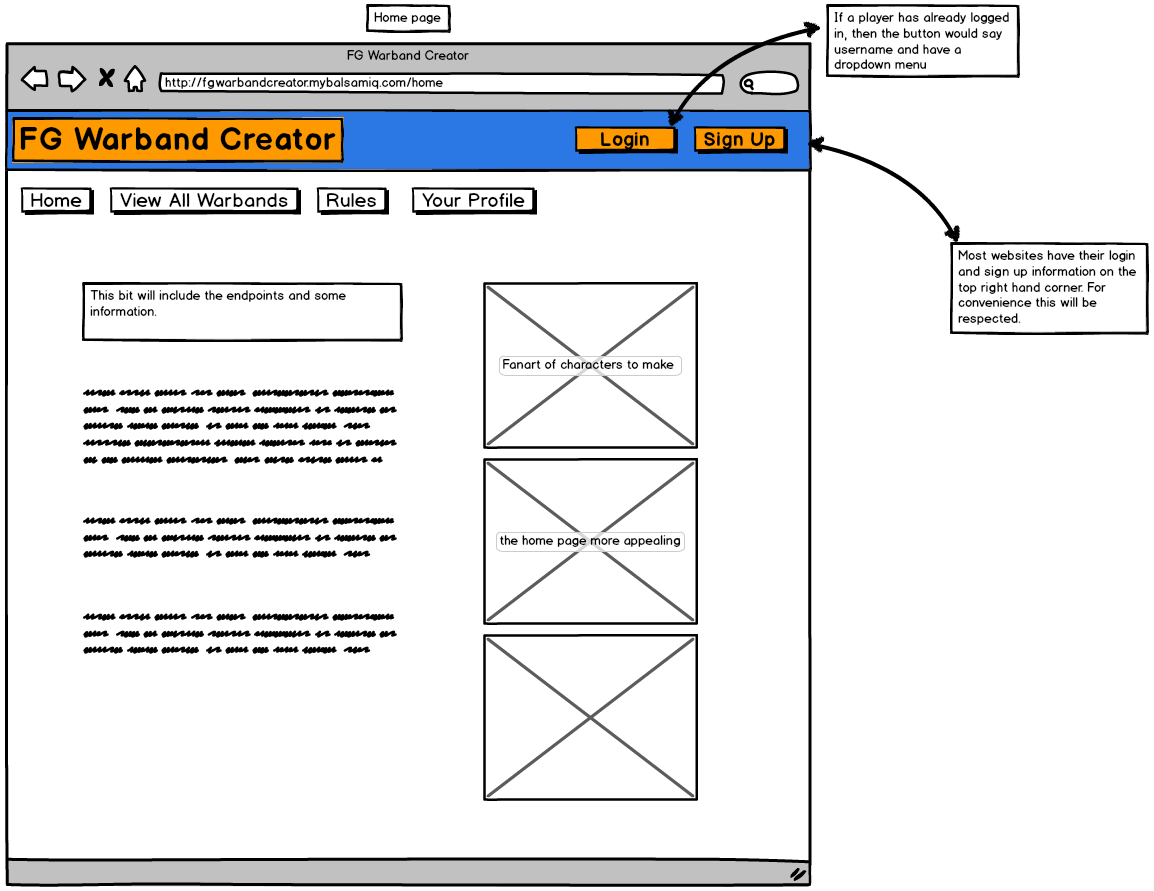
\includegraphics[width=1\textwidth]{img/home}
 \label{fig:3}
 \caption{New ``Home'' page.}
\end{figure}

To make the home page visually appealing to new and existing users, images of the characters should be added - maybe fighting each other, healing, or whatever the characters are supposed to do. The home page should also feature some information, like links to the game's official website, or where to buy the necessary 20 sided dice to play the game. A text section should also explain what is the website, and what it is not. 

For a user that has already logged in, the buttons on the top right corner would be a dropdown menu with the user's username and a ``Log out'' button (respectively). The dropdown menu contains links to ``Your Profile'', your chat, general information, settings, and to delete your account.

\begin{figure}[h!]
 \centering
 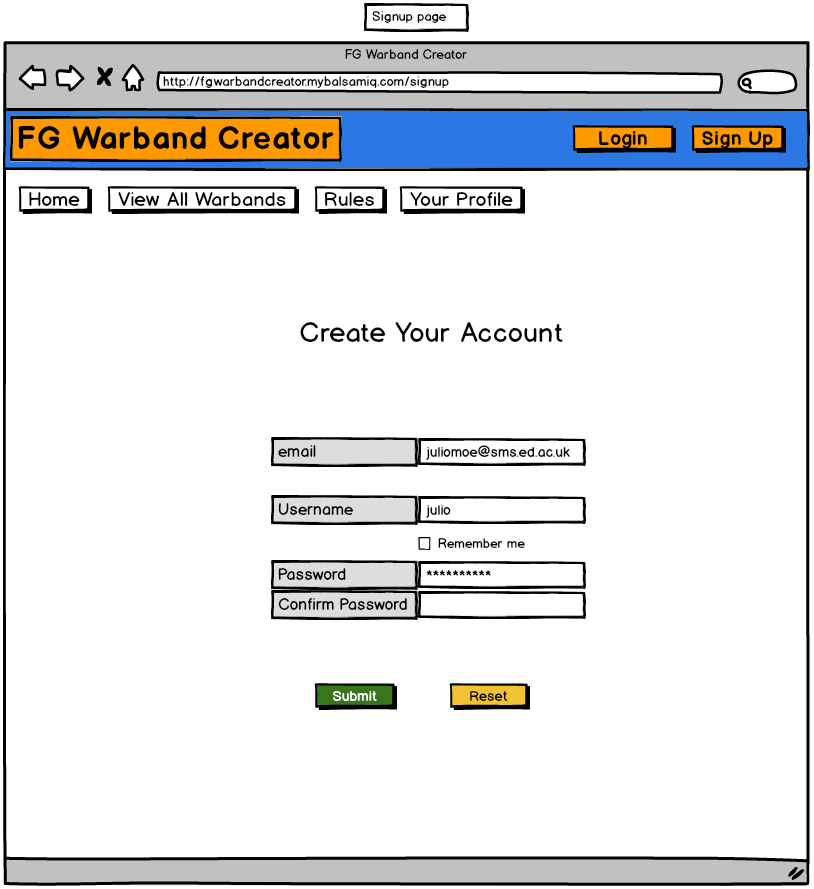
\includegraphics[width=0.8\textwidth]{img/signup}
 \label{fig:4}
 \caption{``Sign up'' page.}
\end{figure}

The next page that a new user would be interested in is the ``Sign up'' page. This is shown in fig.~4. The only information that is asked is the username (that is checked against previously created usernames for uniqueness), a password, an associated email (in case of forgotten password). The ``Remember me'' button to keep the username in auto-fill settings is also included. 

In case of a returning registered user, the first page they would be exposed to after the home page is the ``Login'' page. This is very simple and shown in fig.~5. To avoid difficulties for users that do not use the web application they can use their email or username indistinctly. The ``Remember me'' button is also included. Finally, the common ``Forgot your password?'' is also part of the ``Login'' page.

\begin{figure}[h!]
 \centering
 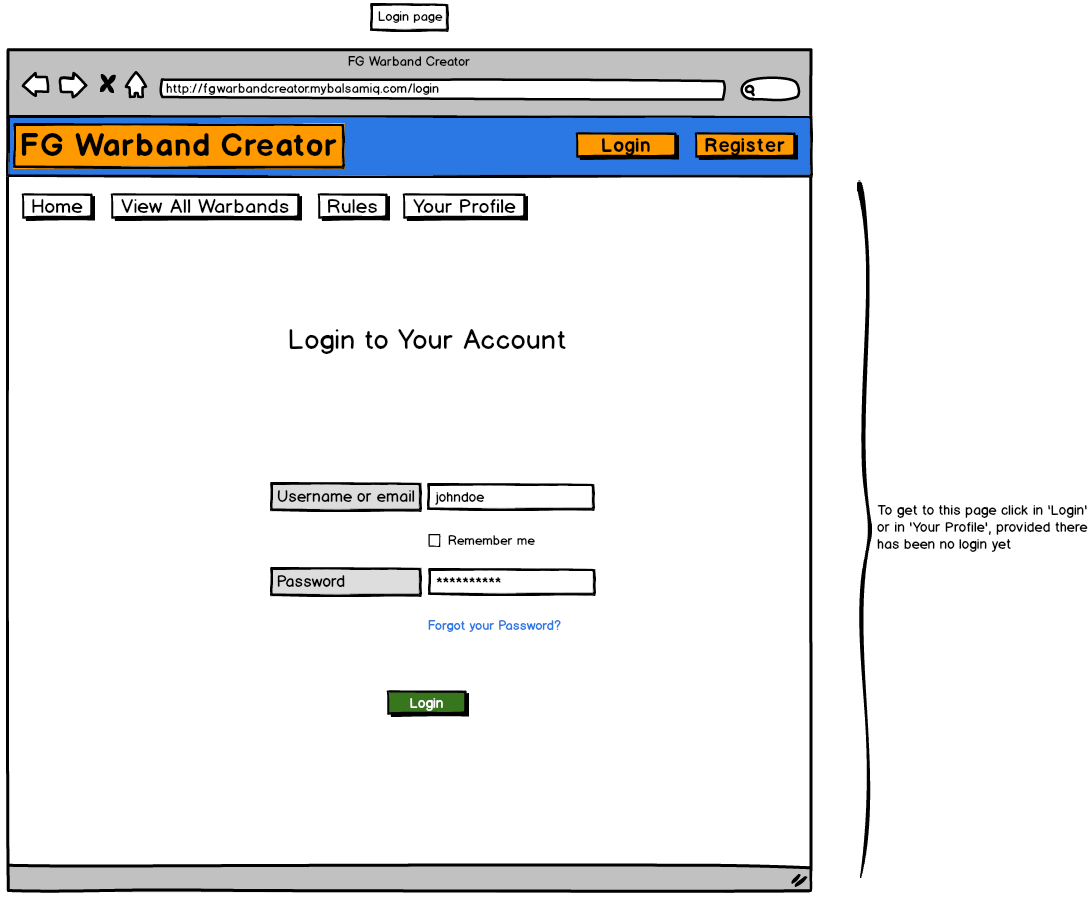
\includegraphics[width=1\textwidth]{img/login}
 \label{fig:5}
 \caption{``Login'' page.}
\end{figure}

These were the bulk of the decisions regarding UI and design to address the problem of multiple user support. In what comes next, the framework supporting multiple users will still be used (and a few comments and images will be used).

\subsection{Confirmation Messages and More}

When a returning user opens their profile page they see their warbands in a table that shows the warband's names and their currency and two options (edit and delete). Pressing the latter shows a confirmation message explaining that the decision is not reversible. This is intended to prevent the accidental deletion of user's warbands. This is shown in fig.~6. The previously mentioned dropdown menu with the username on the top right corner is included. Finally, a ``Create New Warband'' button is placed in the web page.

\begin{figure}[h!]
 \centering
 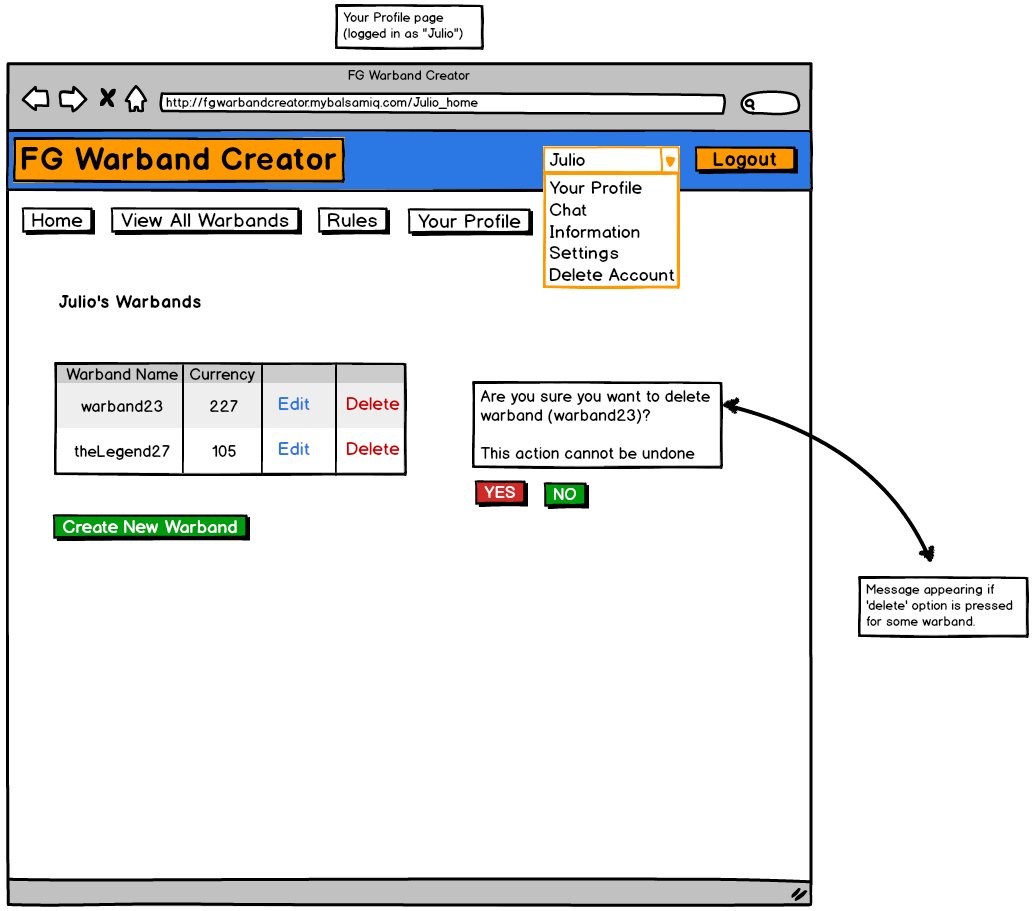
\includegraphics[width=1\textwidth]{img/profile}
 \label{fig:6}
 \caption{``Your Profile'' page.}
\end{figure}

Part of the problems regarding error messages are related to an inappropriate handling of the amount of available credits. The code needs to be fixed so that the number of credits left is actually representative of the warband's remaining credits (account for the Captain and Ensign's weapons). And the design must include the value of each weapon so that the user remembers that they are also considered when calculating the warband's remaining credits. 

The next step would be to allow the user to add members to the team only if their number of credits allows them (without submitting the warband). This is seen in fig.~7, where, with only 45 credits left, the possible warband's members that can be added without leaving a negative number of credits is limited. 

\begin{figure}[h!]
 \centering
 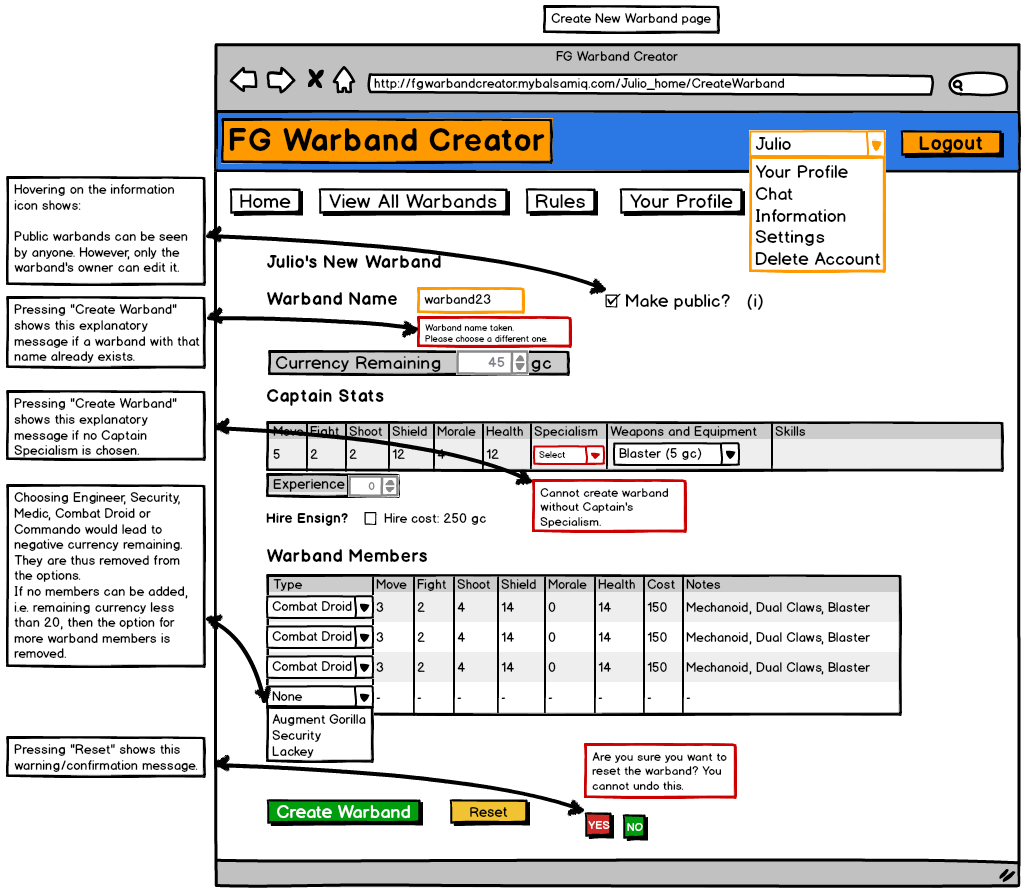
\includegraphics[width=1\textwidth]{img/create_restricted}
 \label{fig:7}
 \caption{``Create New Warband'' page.}
\end{figure}

Figure~7 also shows what happens when a user attempts to create a warband without a Captain Specialism. The current application gives the generic error message for this. The proposed solution is to show a warning message when the user tries to create such a warband and leaving the user in the ``Create New Warband'' page. 

A similar message is used to alert the user that a warband with the desired name already exists. Finally, the reset button also has a confirmation message, for the chance that the user simply pressed the wrong button. A colour coding is also used in this message to try to be user-friendly (making the ``yes'' button red and the ``no'' button green). Finally, the ``Make public?'' tick is also included so that the functionality of viewing other people's public warbands is made available. 

Another simple change to the previous application is to change from ``Apprentice'' to ``Ensign'' as the game calls it - the price for the Ensign is also modified. The associated player name needs not be added, since it is that of the user who is creating the warband.

The way with which new warband members are added is also modified. As it can be seen in fig.~7, a slot for a new member is opened only if the previous has been filled. Even though it is not shown in fig.~7, once the limit for members is reached, a new slot would not be opened. This would also serve as a prevention for teams with more than 10 members. Once the process of creating the new warband is completed the user is redirected to its profile page. There he can decide what to do next. 

Regarding the editing warbands problems, some of these are problems with the code and others are design problems. Problem 3.(a,b), for example, is a problem with the code and will be addressed in the next report. However, regarding the removal of warband members, this is something that cannot be undone, so an warning/confirmation message is included following the format shown above (it can also be seen in fig.~8). A small section of the page is dedicated to the exchange of Experience points of both the Captain and the Ensign towards improving some of their abilities (shown in a dropdown menu). To prevent users of attempting to improve abilities that have already reached their maximum value, those options are removed from the dropdown menu.

\begin{figure}[h!]
 \centering
 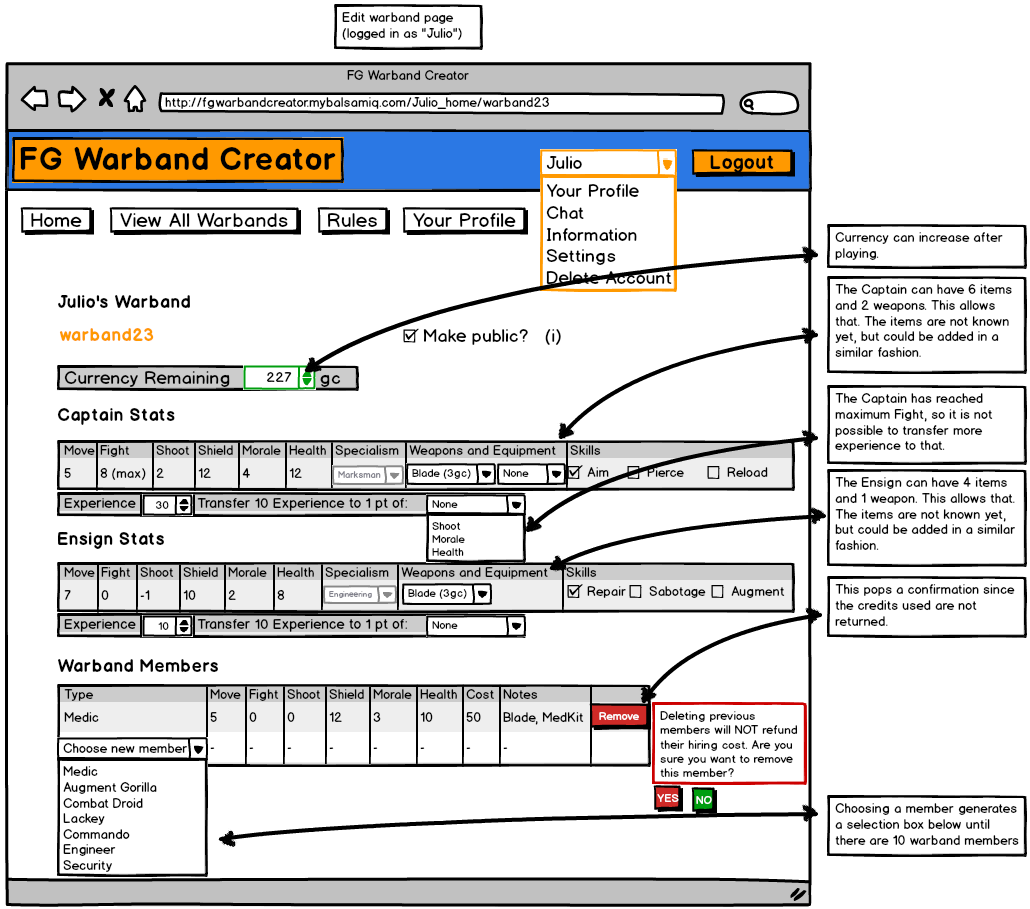
\includegraphics[width=1\textwidth]{img/edit_restricted}
 \label{fig:8}
 \caption{``Edit Warband'' page.}
\end{figure}

The new ``Edit'' page allows users to increase the amount of credits in their warbands, which is one of the game's requirements that was neglected in the given interface. Additionally, users can also add a second weapon for their Captain - however, the equipment or items that they can acquire is unknown so this issue was not addressed. The format for adding warband members is the same as for the ``Create'' page. Finally, the button for removing warband members is linked to a warning message since, when editing a warband, the removal of a member will not refund the credits necessary to hire said member.

The ``View all Warbands'' page does not allow users that do not own the public warbands to modify them in any way, but only view them. This can be shown in fig.~9, as all the fields are greyed out.

\begin{figure}[h!]
 \centering
 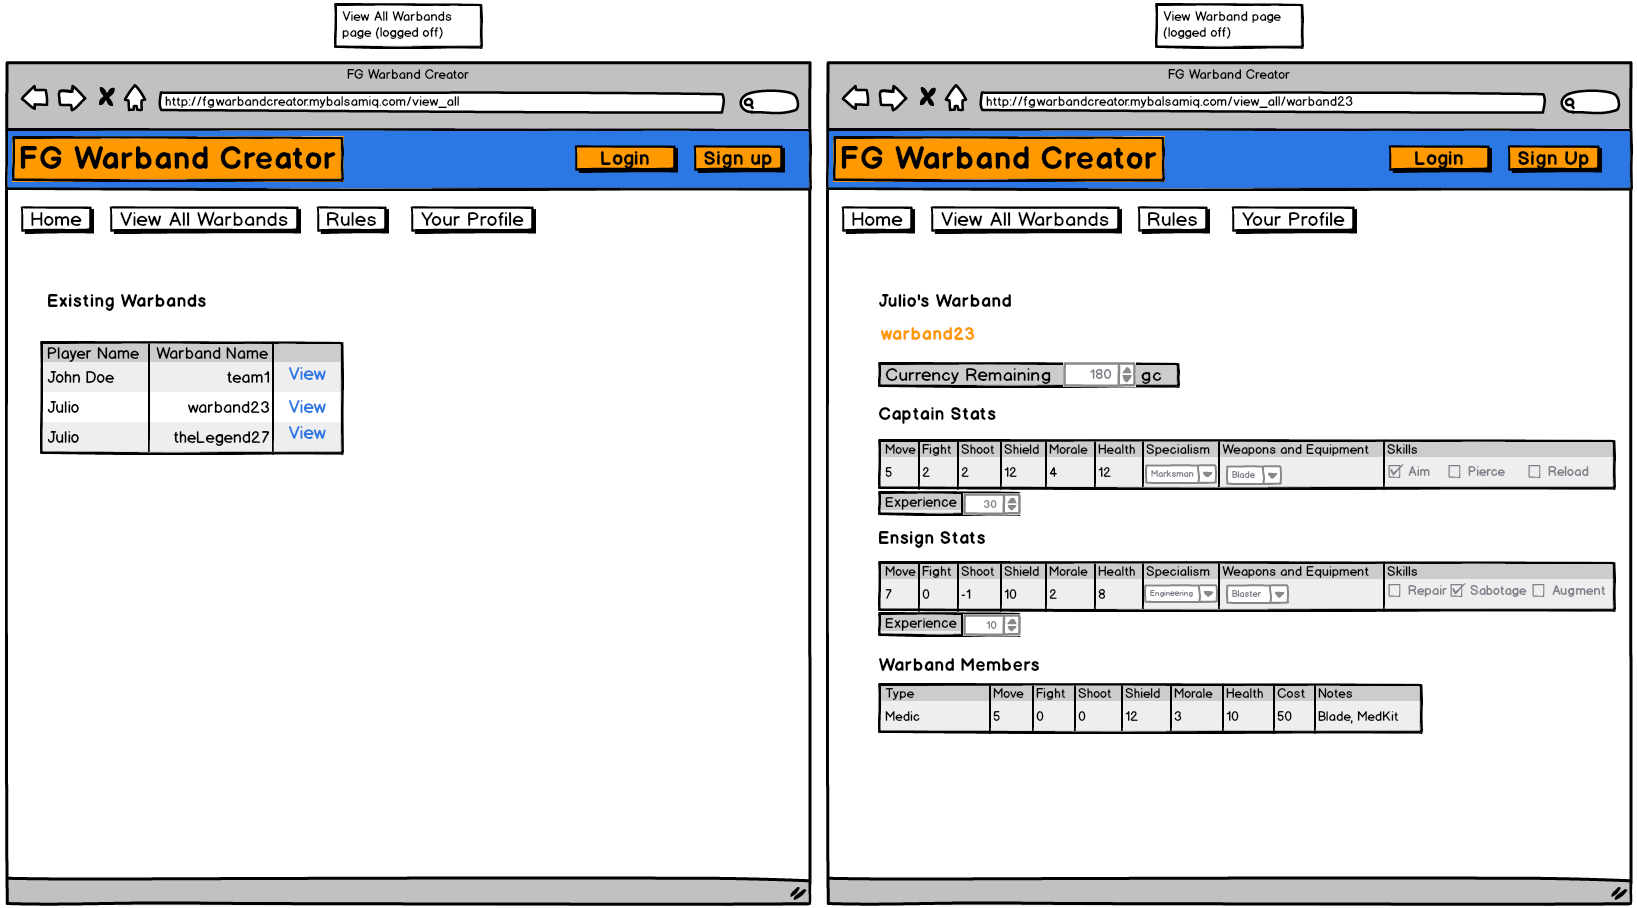
\includegraphics[width=1\textwidth]{img/view_all}
 \label{fig:9}
 \caption{``View all Warbands'' page for logged off users and a public warband under display.}
\end{figure}

As it was mentioned previously, it would be beneficial to the players of this fictitious game to be able to talk to other players so that they can try to get together in real life with their miniatures and their 20 sided dice. This can be implemented once that the web application's users have entered their login credentials and have a username and email associated to them. Using these a chat can be implemented and an link to contact other players is shown in the ``View all Warbands'' page (only for users that have logged in) as it is shown in fig.~10. This also acts as an incentive for players to mark their warbands as public. The messages that a player receives appear as a notification next to their username and can be accessed by clicking ``Chat'' in the dropdown menu on the top right hand corner of the web page.

\begin{figure}[h!]
 \centering
 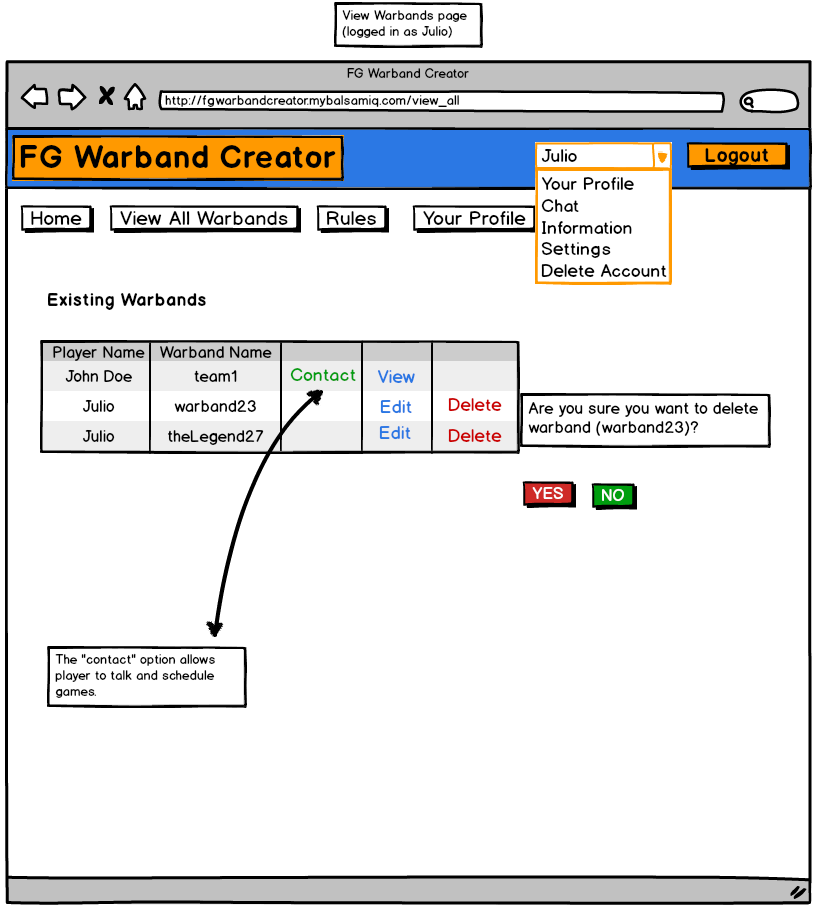
\includegraphics[width=0.8\textwidth]{img/view_all_loggedin}
 \label{fig:10}
 \caption{``View all Warbands'' page for logged in users.}
\end{figure}

\section{Summary of Design Choices}

To solve the problems laid out in section 2 a series of carefully thought out design choices were made. First of all, a multiple user interface was adopted. It follows most website's design decisions regarding the position of the Login, Sign up, Logout and user options (top right hand corner). It also allows people who do not have an account to view other player's public warbands, and also see all the information regarding the game - for example the game's rules. This could hopefully help lure more users into the refurbished platform.

The given version of the website was a very unfriendly, hard to navigate, mess. Several design choices were laid out with the hopes that someone can arrive at the website and, without having to use external buttons or address bars can navigate easily through it. To do this a fixed position menu is placed that allows access to the ``Home'' page, ``View all Warbands'', ``Rules'', and ``Your Profile''. Additionally, on the top right hand corner more navigation options are included for users that have an account. 

To make the web application more friendly the error messages will be completely removed and substituted with friendly messages with confirmation buttons. The website will also be coloured and this will be used to colour code certain options (like making delete buttons red).

Users trying to create new warbands will no longer have to deal with problems like obnoxious error messages or the uncertainty on whether or not their warband was actually created. Including a short message of ``Your warband was successfully created'' and redirecting the user to their profile page will provide some peace of mind. Keeping an accurate account of new warbands, as well as warbands being edited, it will be easier for the user to create or edit a warband without any complications. 

By preventing the user to be able to attempt to make a warband with more than 10 members or with negative number of credits, the user's experience while using the application will be more relaxed and they will likely want to come back to it. A small addition to the ``Edit'' page was also made in order to transfer Experience to points in abilities. This was previously not rigorous and had no control over surpassing the maximum values for each ability - some abilities that cannot be improved provided the option to increase without limit! 



\section{UI Evaluation Plan}

A large number of changes have been mocked-up in this report. It is safe to consider them necessary additions to the project. Nevertheless, it is possible that the solutions proposed are not the best alternative for fixing the exposed problems. It can also be the case that there are multiple problems with the given application that are not mentioned in this report. All these options are real and can be considered by having more people look at the problem and at the solutions. 

Assuming that there are not 30 other people working on this problem, i.e. the rest of the Software Development course, very few people actually know about this web application. Before anything is shown to outside parties, it is important to talk about the proposed solutions with the people paying for the product. This is ideal as it avoids a serious problem. As it was mentioned in class, when a developer goes to the employer with a functional front-end to ask design questions, the latter might have the erroneous perception that the product is close to being finished, and it is receiving final touches before delivery. However, since we would be going to the employer with merely a mock-up of the design that we want to implement, then this problem is non-existent, and after having an OK from the employers we could start working on a functional front-end.

So, the first step in evaluating the decisions that have been made to improve the given web application will be to show them to the employers (provided that this is a one-person project, otherwise the first step would be to talk about the proposed solutions with workmates). They will be able to spot even more requirements that the game has and that are not represented in the proposed mock-up. After addressing what should be a few missed problems and incorporating them to the improved mock-ups, the first stage of the evaluation plan will be completed. 

Since there is no front-end yet, and a working (improved) product does not exist it would be hard to do something like on-line questionnaires to obtain feedback of the functionality of the web application. However, it would be possible to talk to people of different backgrounds about this fictitious game and then, after making sure they understand what is the game and what are the restrictions that it has to go through the mock-up created for the improved web application. Doing this with with people from the MSc. in HPC would return technical information probably valuable at improving the user interface for the multiple user support (which is a very important component to the game in a large scale). 

Going to people that frequent the ``Warhammer'' store on High Street, Edinburgh will help in providing information regarding how to attract players of similar skirmish table top games with miniature figures. Listening what they want to see in a website to build squads might be very valuable as they could accurately represent the market that the game is trying to probe into. 

Asking people that have no interest in software development or in table top games can also be very valuable, given that they are internet users (pick people under 70 to avoid that they are not). They will provide the most insight regarding how accessible the application is, its user-friendliness and what could change to improve the experience that they are perceiving. This might be dangerous, though, if they hold no interest in the game or the development of the application they might not be paying attention when they are listening/reading to the stipulations of the game and might ask for illegal things (on the game's point of view). It is important to take that into consideration.

Finally, and after implementing the information acquired from these sources it could be a good idea to turn to the internet with an appropriate framework of questionnaire. This can be done in a similar manner and possibly trying to find people who are actually playing the fictitious game and hearing what it is that they would expect from such a platform. If anyone in the world should like the end product of this project it is the people who will use it. Hearing what they have to say about the existing application and how they would improve it can be very valuable. For example, such a community could be great at providing the fanart for the website's home page.

\newpage


\begin{thebibliography}{100}

\bibitem{soft_dev} Software Development. {\em Software Development Coursework.} University of Edinburgh. 2017.

%\bibitem{ref:bloggs} F.Bloggs. {\em 1993 Latex Users do it
%in Environments} Int. Journal of Silly Findings. pp 23-29.

\end{thebibliography}


\end{document}

